\chapter{Methodology} % Main chapter title

\label{Chapter4} % Change X to a consecutive number; for referencing this chapter elsewhere, use \ref{ChapterX}

\section{Phenanthrene Parameterization}\label{parame}

The two parameterization strategies for molecules with aromatic rings described in section \ref{parsaft} were implemented for phenanthrene. For both of them, only vapor pressure data \cite{pvphen} were used due to the unavailability of saturated liquid density. We did not estimate the attractive exponent, $\lambda _{a}$. Instead, the value of six was given to it due to its high correlation with the repulsive exponent. The parameterization with the ring equation of \citeonline{muller2017} was done with the number of segments equals to five and the following geometry, since this level of coarse graining was also used for a similar molecule (anthracene) in the original paper:
\begin{figure}[th]
	\centering
	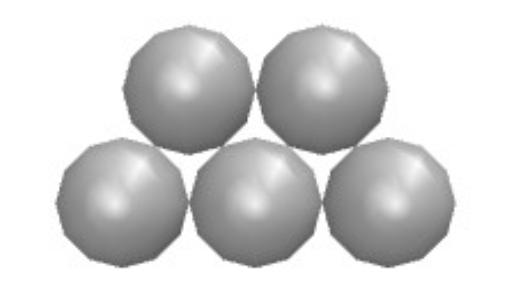
\includegraphics[width=0.25\linewidth]{Figures/fen5}
	\caption{Geometry for $m_{s}=5$}
	\label{fig:fen5}
\end{figure}

The minimization was done using the Particle Swarm Optimization (PSO)  method \cite{pso} with the following objective function:
\begin{equation}
\min\limits_{\sigma,\epsilon,\lambda_{r}} F_{obj}(\sigma,\epsilon,\lambda_{r})= \sum_{i=1}^{N_{p}} \left(\frac{P_{v}^{SAFT}(T_{i},\sigma,\epsilon,\lambda_{r})-P_{v}^{exp}(T_{i})}{P_{v}^{exp}(T_{i})} \right)^2
\label{eqn:fobjm}
\end{equation}

Here, $P_{v}^{exp}$ is the experimental vapor pressure and $P_{v}^{SAFT}$ is the vapor pressure obtained with SAFT-VR Mie EoS. We used the routine proposed by  \citeonline{smithbook} to calculate the bubble point with the EoS. The resulting  parameters ($\sigma$, $\epsilon $ and $\lambda _{r}$) of Eq. \eqref{eqn:fobjm} are the final force field parameters used in molecular simulations. 

The parameterization with the \citeonline{lafitte2012} ring equation was done with $m_{s}=3$ so every bead would represent one aromatic ring:

\begin{figure}[th]
	\centering
	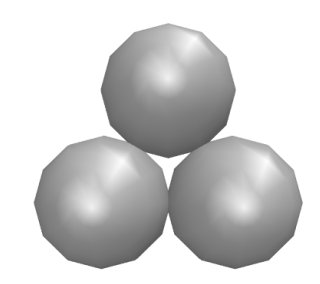
\includegraphics[width=0.15\linewidth]{Figures/fe3}
	\caption{Geometry for $m_{s}=3$}
	\label{fig:fen3}
\end{figure}

The first part of the estimation followed the same procedure described above for the \citeonline{muller2017} equation. As explained in section \ref{parsaft}, the \citeonline{lafitte2012} equation requires the estimation of correction factors $c_{\sigma}$ and $c_{\epsilon}$ (Eqs. \eqref{eqn:csigma} and \eqref{eqn:ceps}). We then estimated these parameters using the PSO method with Eq. \eqref{eqn:fobjla}. In this equation, the vapor pressures and saturated liquid densities from molecular simulations were obtained using the Gibbs Ensemble Monte Carlo method on the NVT ensemble  (section \ref{gemc}).

The boxes for the GEMC-NVT simulations were generated inserting 400 molecules of phenanthrene into the liquid box and 100 molecules of phenanthrene into the vapor one using the Playmol package \cite{playmol} integrated with the Packmol package \cite{packmol}. Initial densities of each box were equal to the saturated densities found with the SAFT-VR Mie Eos in order to avoid the migration of all molecules to a single phase throughout the simulation. The GEMC-NVT simulations were carried using the Cassandra software \cite{doi:10.1063/1.3644939}, developed to perform Monte Carlo simulations. The equilibration and production times lasted around  $10^{4}$ and $5 \, 10^{4}$ MC cycles respectively. Each MC cycle corresponded to $10^3$ rotation trials, $10^3$ translation trials, $10^2$ molecule insertion trials, $10^2$ molecule deletion trials, and 10 volume exchange trials. The cut off distance was equal to $20 \, \hat{A}$ and we did not use long range interactions. The saturated vapor density ($\rho_{vap}$), the saturated liquid density ($\rho_{liq}$), and the vapor pressure ($P_{v}$) were sampled at each 100 MC cycles. Later, these data were divided in five blocks to calculate the averages and standard deviations. With the correction factors found after the estimation with the simulation data, we calculated with Eqs. \eqref{eqn:simsigma} and \eqref{eqn:simeps} the $\sigma$ and $\epsilon$ parameters, which are the ones to be used in molecular simulations.


\section{Solvation Free Energy Calculations}\label{solvme}

Using the parameters for phenanthrene estimated with the \citeonline{muller2017} aproach  and the available SAFT-$\gamma$ Mie force field parameters, we carried out molecular dynamic simulations in order to estimate solvation free energy differences. The chosen software package to perform the simulations was the Lammps package\cite{lammps}. In it, the motion equations were integrated with the velocity-Verlet algorithm \cite{verlet} with a time step of 2 fs. As required by the coarse grained model,  molecules were treated as rigid bodies. The thermostat and the barostat were the Nose/Hoover with chains with a damping factors of 100 and 1000 time steps respectively. Electrostatics interactions are not explicitly accounted by the SAFT-$\gamma$ Mie force field, hence there were no shifting of forces or long range corrections. The potential cutoff was equal to 20 $\dot{A}$ \cite{muller2017} with a neighbor skin of 2 $\dot{A}$. The initial configurations of the  solvated systems were also generated using the Playmol package integrated with the Packmol package. For the binary mixtures, one molecule of solute and a varying number of solvent molecules- 700 molecules of toluene, 700 molecules of octanol, 1024 molecules of hexane, 3000 molecules of water - were randomly added to a cubic box. The simulations to study solvation free energy of phenanthrene in a mixture of toluene and carbon dioxide were done with different weight fractions of carbon dioxide. The  system consisted of one molecule of phenanthrene for all the fractions and 123 molecules of $CO_{2}$ and 618 molecules of toluene for $w_{CO_{2}} = 0.087$; 166 molecules of $CO_{2}$ and 589 molecules of toluene for $w_{CO_{2}} = 0.119$; 232 molecules of $CO_{2}$ and 545 molecules of toluene for $w_{CO_{2}} = 0.169$; 380 molecules of $CO_{2}$ and 446 molecules of toluene for $w_{CO_{2}} = 0.289$.

All simulations were performed with the constant temperature and pressure values of 298 K and 1 bar, except the ones containing carbon dioxide. These had the temperature of 298 K and the pressure of the liquid phase equilibrium correspondent to the $CO_{2}$ fraction \cite{co2toliq}. For all the simulations, the initial box was equilibrated at the NPT ensemble for 2 ns, and the resulting configurations were used as the initial configuration of the expanded ensemble simulations. These were carried out with the Lammps user package for expanded ensemble simulations with the Mie Potential developed by our group, available at https://github.com/atoms-ufrj/USER-ALCHEMICAL. 

During these expanded ensemble simulations, the sampling of a new alchemical state was tried at every 10 MD steps. In order to define the optimal values of $\lambda$ and $\eta$ related to each state, short trials simulations, having around 9 ns of production time, were carried out. In the first simulation, the group of $\lambda$ was chosen arbitrarily and the $\eta s$ were set to zero or were given the values of the ones found for similar pairs solute-solvent. The subsequent group of $\eta$ were estimated  with the flat histogram approach (Eq. \eqref{eqn:weight}). We then did another trial simulation with the new weights. The results of this simulation were used to optimize the group of $\lambda s$ by minimizing the number of round trips, as described in section \ref{ee}. The $\eta s$ correspondent to the newest group of $\lambda s$ were interpolated linearly from the free energy differences. With the final values of $\eta$ and $\lambda $ defined for each mixture, larger simulations with a production time of 20 ns were carried out. 

Since the force field used considers that the beads don't have charges, there are no Coulombic interactions, and Eq. \eqref{eq:freesolv} becomes equal to $\Delta G_{3 \rightarrow 4} $. The post processing method used to effectively calculate free energy differences with the potential energies obtained from the expanded ensemble simulations was the Multisate Bennet Acceptance Ratio (MBAR), described in section \ref{mbar}. The software alchemical-analysis \cite{klimovich} was utilized to obtain the $\Delta G_{solv}$ with MBAR and to assess the quality of the results. After the first estimations, we realized the need of the binary interaction parameter of Eq. \eqref{eqn:epsmix} for pairs with water as solvent. Hence, we estimated  $k_{ij}$ for these pairs and, for all the other pairs,  $k_{ij}$ was set to zero. The estimation was done by performing trial  expanded ensemble simulations in three values of $k_{ij}$, as suggested by \citeonline{ervik20162}. With the $\Delta G_{solv}$ obtained with these simulations, we did a linear fit to obtain the refined value of the parameter. We used this strategy because the estimation with SAFT VR Mie EoS gave poor results for the solvation free energies.

